\begin{frame}[fragile]{Que fait ce programme ?}

  \vspace{-2mm}
  \begin{tikzpicture}
    \fill[alertColor!20, rounded corners] (3.5,3.65) rectangle (8,4);
    \draw[alertColor] (10,3.85) node{//$T_{A}$};

    \fill[exampleColor!20, rounded corners] (3.5,2.65) rectangle (8,3);
    \draw[exampleColor] (10,2.9) node{//$T_{G}$};
    \draw (5,5.18) node{\begin{minipage}{5cm}\begin{lstlisting}[numbers=none]
public record Friend(String nom) {
  public synchronized void salute(Friend friend) {
    System.out.println(nom + " salutes " + friend.nom);
    friend.answer(this);
  }
  
  public synchronized void answer(Friend friend) {
    System.out.println(nom + " answers to " + friend.nom);
  }
  
  public static void main(String[] args) {
    var alphonse = new Friend("Alphonse");
    var gaston = new Friend("Gaston");
    new Thread(() -> 
      alphonse.salute(gaston)
    ).start();
    new Thread(() -> 
      gaston.salute(alphonse)
    ).start();
  }
}
\end{lstlisting}\end{minipage}};
  \end{tikzpicture}
  \vspace{-2mm}
\begin{citing}
\jitem \lstinline{tp1/Friends.java}
\end{citing}
\end{frame}

\begin{frame}[fragile]{Exemple d'exécution}
  \begin{lstlisting}[numbers=none]
public synchronized void salute(Friend friend) {
  System.out.println(nom + " salutes " + friend.nom);
  friend.answer(this);
}

public synchronized void answer(Friend friend) {
  System.out.println(nom + " answers to " + friend.nom);
}
  \end{lstlisting}
  
\scalebox{.6}{
      \begin{tikzpicture}

        \draw[alertColor, fill=alertColor!10, rounded corners] (15,5.6) --  (1, 5.6) -- (1,4.4) -- (15,4.4);
        \draw[exampleColor, fill=exampleColor!10, rounded corners] (15,3.6) --  (2.1, 3.6) -- (2.1,2.4) -- (15,2.4);

        \draw[structure ,   -latex] (0,5) node[left]{$T_A$}      -- (16,5);
        \draw[structure,    -latex] (0,3) node[left]{$T_G$}      -- (16,3);

        \draw[alertColor, fill=alertColor!30, rounded corners] (1.1,5.5) rectangle (3.3,4.5);
        \draw[exampleColor, fill=exampleColor!30, rounded corners] (2.2,3.5) rectangle (4.4,2.5);

        \draw[alertColor]   (2.2,5) node{alphonse.lock};
        \draw[exampleColor] (3.3,3) node{gaston.lock};

        \draw[structure, fill=structure!30, rounded corners] (3.4,5.5) rectangle (5.4,4.5);
        \draw[structure, fill=structure!30, rounded corners] (4.5,3.5) rectangle (6.5,2.5);

        \draw[structure] (4.4,5) node{println};
        \draw[structure] (5.5,3) node{println};

        \draw[exampleColor, fill=exampleColor!20, rounded corners] (15,5.5) --  (5.5, 5.5) -- (5.5,4.5) -- (15,4.5);
        \draw[alertColor, fill=alertColor!20, rounded corners] (15,3.5) --  (6.6, 3.5) -- (6.6,2.5) -- (15,2.5);
 
        \draw[exampleColor, fill=exampleColor!30, rounded corners] (15,5.4) --  (5.6, 5.4) -- (5.6,4.6) -- (15,4.6);
        \draw[alertColor, fill=alertColor!30, rounded corners]     (15,3.4) --  (6.7, 3.4) -- (6.7,2.6) -- (15,2.6);

        \draw[exampleColor] (6.7,5) node{gaston.lock};
        \draw[alertColor]   (7.8,3) node{alphonse.lock};
\end{tikzpicture}
}
\begin{alertblock}{À ce point :}
  \begin{itemize}
  \item $T_A$ est bloqué par $T_G$ sur le verrou de \lstinline{gaston}
  \item $T_G$ est bloqué par $T_A$ sur le verrou de \lstinline{alphonse}
  \end{itemize}
\end{alertblock}
  
\end{frame}

\begin{frame}{Interblocage circulaire}
    \begin{block}{Deadlock}
      Situation  d'\alert{interblocage circulaire}  où  des threads  attendent
      entre eux la libération de ressources avant de continuer leur exécution.
    \end{block}
      \begin{center}
        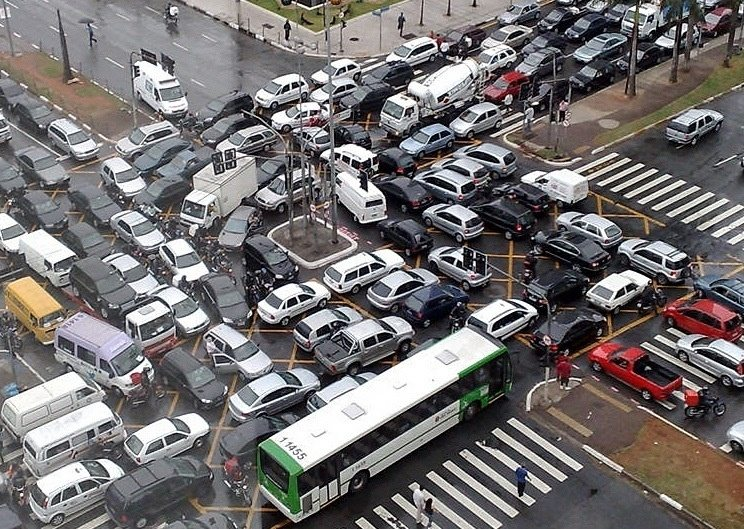
\includegraphics[height=4cm]{deadlock}
      \end{center}
\end{frame}

\begin{frame}
  \frametitle{Une solution pour éviter les deadlocks}
\vFill
  \begin{alertblock}{Composition}
    Des deadlocks peuvent se produire quand plusieurs verrous sont utilisés.
  \end{alertblock}
\vFill
  \begin{block}{Théorème}
    \begin{itemize}
    \item Supposons qu'il y a un ordre sur les verrous $v_1 \le v_2 \le \dots \le v_n$.
    \item Supposons qu'aucun thread ne cherche à obtenir $v$ alors qu'il possède déjà $v'$ avec $v\le v'$.
    \item Alors l'exécution ne comporte pas de deadlock.
    \end{itemize}
  \end{block}

\vFill
  \begin{alertblock}{En TD}
    Utilisez le théorème ci-dessus pour résoudre le problème du dîner des philosophes
  \end{alertblock}
\vFill
\end{frame}

\begin{frame}{Situation de famine}
  \vFill
  \begin{block}{Starvation}
    Situation où un ou  plusieurs threads n'ont \alert{jamais accès}
    à la ressource demandée.
  \end{block}
  \vFill
  \begin{center}
    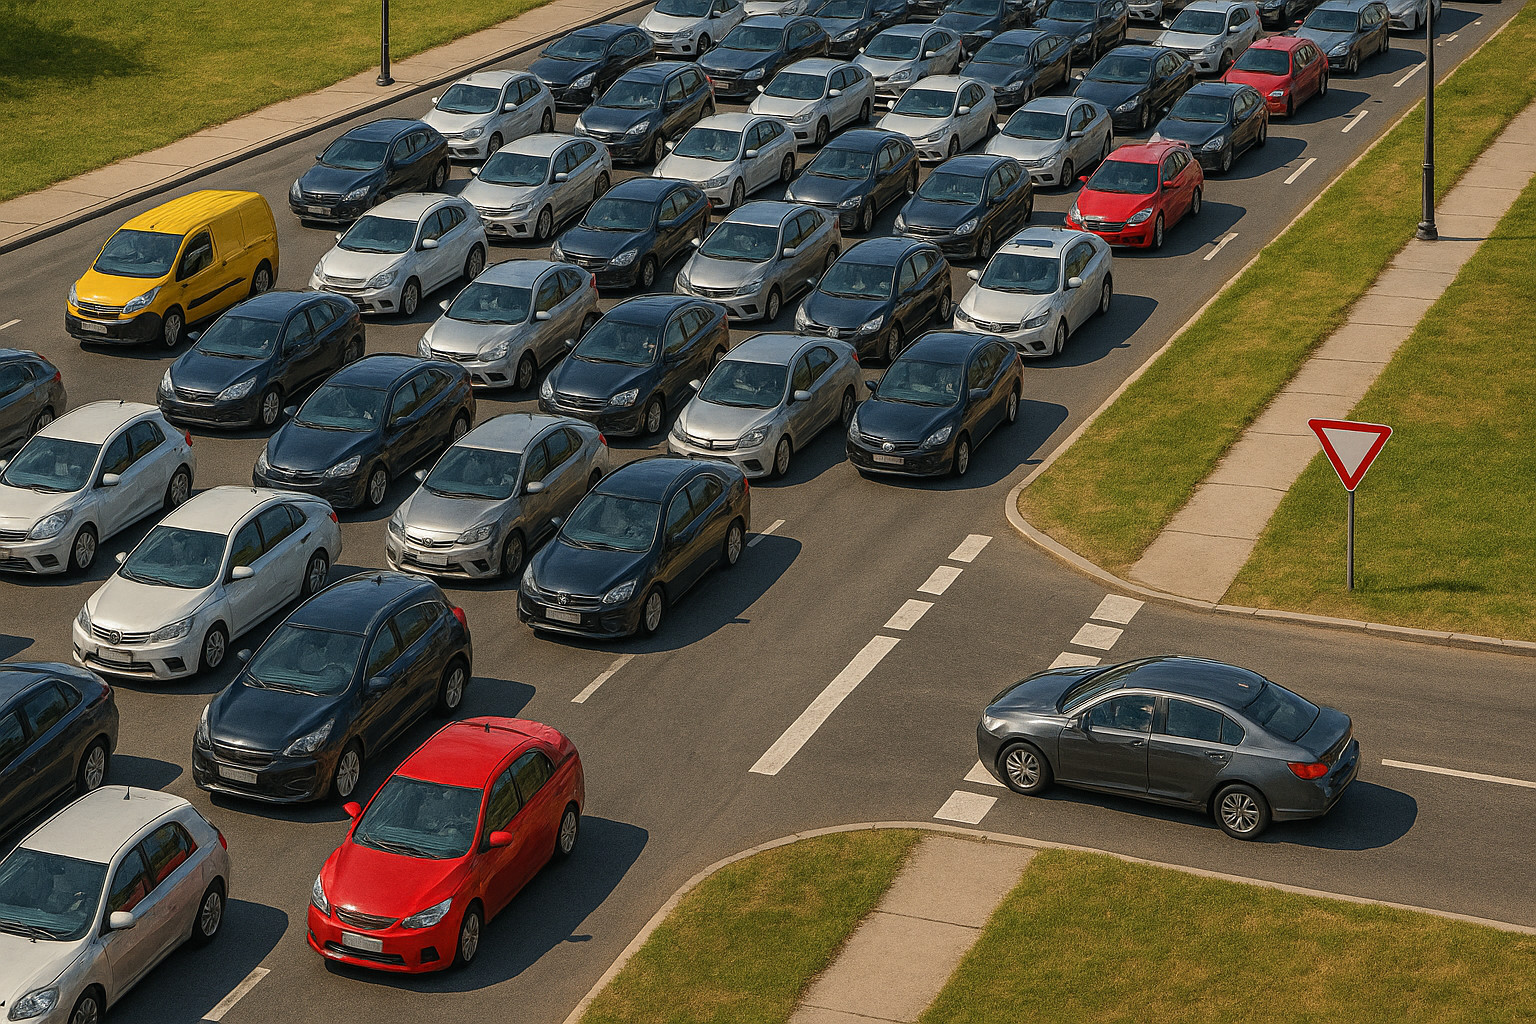
\includegraphics[height=4cm]{starvation}
  \end{center}      
  \vFill
  \begin{alertblock}{En TD}
    Observez les problèmes de famine dans le problème des toilettes unisexes.
  \end{alertblock}
  \vFill
\end{frame}

